\section{Applications}

\subsection{Privacy-preserving pools}
\noindent Barring some exceptions, most blockchains allow public access to transaction details. These could include the source wallet, destination wallet, the tokens transferred, and other potentially sensitive information. When endowed with zero-knowledge properties, modern SNARKs can help address this issue as needed. A helpful solution could involve someone depositing into some liquidity pool from wallet $A$, then withdrawing some portion of that deposit to wallet $B$ without revealing any deposit details (beyond the amount), including the link between wallets $A, B$. Tornado cash smart contracts make this possible by keeping a merkle tree of deposit commitments. When a user deposits into the pool, they create a commitment to their deposit derived partially from secret data only they should know. This commitment is inserted into the tree. When the same user goes to withdraw, they must provide a groth16 proof that their deposit commitment is indeed present in the tree. The homogeneous nature of the computation being verified -- namely, the recursive hashing of nodes to the tree root -- makes groth16 suitable for this use case.\\

\begin{figure}[ht]
\centering
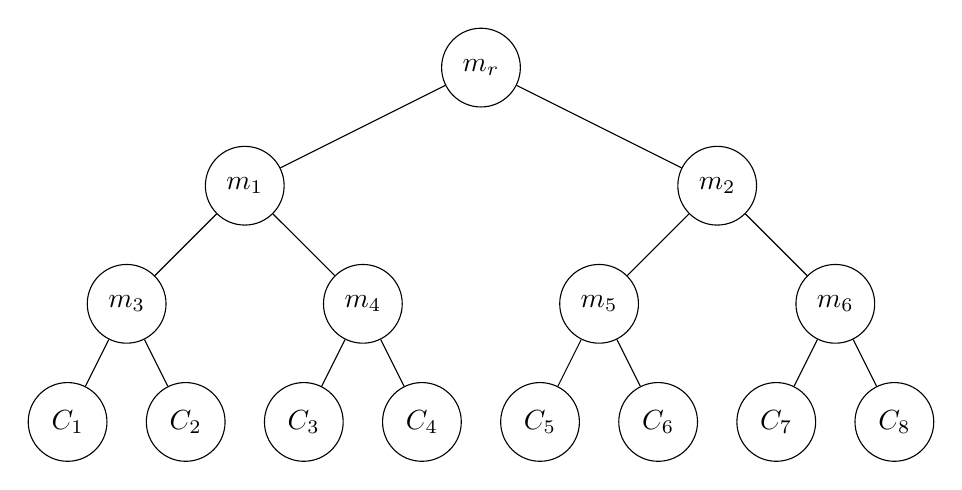
\begin{tikzpicture}[
    level 1/.style={sibling distance=60mm},
    level 2/.style={sibling distance=30mm},
    level 3/.style={sibling distance=15mm},
    every node/.style={draw, circle, minimum size=10mm}
]
    % Root node
    \node {$m_r$}
        % Level 1
        child {node {$m_1$}
            % Level 2
            child {node {$m_3$}
                % Level 3
                child {node {$C_1$}}
                child {node {$C_2$}}
            }
            child {node {$m_4$}
                % Level 3
                child {node {$C_3$}}
                child {node {$C_4$}}
            }
        }
        child {node {$m_2$}
            % Level 2
            child {node {$m_5$}
                % Level 3
                child {node {$C_5$}}
                child {node {$C_6$}}
            }
            child {node {$m_6$}
                % Level 3
                child {node {$C_7$}}
                child {node {$C_8$}}
            }
        };
\end{tikzpicture}
\caption{Merkle tree of deposit commitments in a privacy-preserving pool}
\label{fig:merkle-tree}
\end{figure}

\noindent If we make a deposit associated with commitment $C_6$ and we want to withdraw later, we would have to construct a proof $\pi$ showing that\\
\begin{itemize}
    \item we know the inputs (secret included) that produce $C_6$
    \item we know the merkle authentication path involving $C_5, m_6, m_1$ that would yield $m_r$.
    \item we know the secret used to produce a \textit{nullifier hash} which helps to mark $\pi$ as already used so it cannot be replayed
\end{itemize}

\noindent The tornado cash infrastructure includes off-chain components with this functionality. In particular, it contains circuits written in Circom which can be used to generate and verify groth16 proofs of deposit commitment validity.\\

\subsection{Privacy-preserving blockchains}
\noindent discuss UTXO model and proof of membership\\

\subsection{Verifiable Virtual Machines (VVM)}
\noindent So-called ``Zero-knowledge virtual machines'' (zkVMs) have emerged as an elegant solution to settling transaction batches from layer 2 (L2) blockchains on the layer 1 (L1) chain they derive crypto-economic security from. We use the more accurate phrase ``verifiable virtual machine'' (VVM) since succinctness is a higher priority than zero-knowledge in most L2 architectures. To align with real-world use cases like polygon zkEVM, Scroll, and others, we consider a centralized L2 blockchain with a single node that receives transactions, orders them, and creates blocks from them. The node then constructs a SNARK of block validity and sends this proof to a verifier contract on the L1 chain for verification. The SNARK is constructed from a large circuit which must constrain the witness to describe only valid computation paths through the VVM. Since the computation structure can change every time, this calls for use of universal SNARKs, of which PlonK and its variants are popular choices. More concretely, many VVM implementations use circuit domain-specific languages (DSLs) like halo2 to implement the circuits constraining the computation details.\\

\noindent A crucial point of consideration here is that not all computations performed in VVMs are ``SNARK-friendly''; a prime example of this is hash functions like SHA256 which use non-linear or non-algebraic operations like bit mixing. This can cause the circuits constraining this computation to be overly complex and inefficient. To meet this end, lookup-based methods are of great interest here since they can avoid constraining ``SNARK-unfriendly'' operations directly without losing soundness. An example of this is lies in the proof for validity of transaction that called a contract function using \texttt{sha256()}. Instead of constraining the exact sha-256 computation, the prover and verifier would agree on a publicly known table of acceptable inputs and outputs for SHA-256, which the prover commits to as part of the proof. The verifier does not need to know the whole table - they just need to know a commitment to the one considered correct. This can then be compared with what the prover committed to.\\
